\documentclass[a4paper]{jpconf}
\usepackage{graphicx}
\begin{document}

\title{Enabling campus grids with Open Science Grid technology}

\author{Derek Weitzel$^{1}$, Brian Bockelman$^{2}$, Dan Fraser$^{3}$, Ruth Pordes$^{4}$ and David Swanson$^{5}$}

\address{$^{1,2,5}$ University of Nebraska Holland Computing Center, 118 Schorr Center, Lincoln NE 68588 \\
$^{3}$ Argonne National Laboratory, 9700 S. Cass Ave., Bldg 240, Argonne, IL 60439 \\
$^{4}$ Fermilab, MS 369, PO Box 500, Batavia Il 60510 \\
}

\ead{$^{1}$dweitzel@cse.unl.edu, $^{2}$bbockelm@cse.unl.edu, $^{3}$fraser@anl.gov, $^{4}$ruth@fnal.gov, $^
{5}$dswanson@cse.unl.edu }

\begin{abstract}
The Open Science Grid is a recognized key component of the US national cyber-infrastructure enabling scientific 
discovery through advanced high throughput computing. The principles and techniques that underlie the Open Science Grid 
can also be applied to Campus Grids since many of the requirements are the same, even if the implementation 
technologies differ.  We find five requirements for a campus grid:   trust relationships, job submission, resource 
independence, accounting, and data management.  The Holland Computing Center's campus grid at the University of 
Nebraska-Lincoln was designed to fulfill the requirements of a campus grid.  A bridging daemon was designed to bring 
non-Condor clusters into a grid managed by Condor.  Condor features also make it possible to bridge Condor sites into a 
multi-campus grid and we have exploited this capability at the Holland Computing Center as well.

\end{abstract}

\section{Introduction}
A grid is a combination of computer resources from a multiple administrative domains utilized to reach a common goal.
Grids have been successful in accomplishing both homogeneous interfaces and resource pooling at the national level, 
although it has taken much longer to accomplish than originally expected.  At the US national level, there are two large 
grid organizations �- the Open Science Grid (OSG) \cite{pordes2007open} and the TeraGrid \cite{catlett2005philosophy}.  

TeraGrid, by virtue of the high end interconnects and unique designs of its resources, focuses on capability computing 
(e.g. running jobs that cannot run anywhere else). The Open Science Grid focuses on High Throughput Computing (HTC) 
, focussing on tasks that require as much computing power (throughput) as possible over long periods of time \cite
{gridbook-htc}.  This style is typified by ensembles of independent single processor jobs.  Since there is no parallel 
communication between the jobs in a given task, they can be distributed across multiple resources.  This increases 
throughput, the end-goal of HTC.  HTC can use pooled resources mostly interchangeably and as such is well suited to 
distributed and grid computing models.  The OSG has demonstrated its technologies are successful; in Q4 2010, the OSG 
averaged over a 400,000 jobs and a million computational hours a day using HTC.

The HTC style of computing is beneficial for campuses because it can improve utilization across many resources.  The 
principles and techniques the OSG follows are just as powerful at the campus level as they are at the national 
level.  This has been recognized independently in several campus grids across the US, with several implementations; 
these motivations and exemplar implementations are covered in \ref{sec:background}.  In section \ref
{sec:requirements}, we explore the characteristics we will use as a rubric for examining campus grids.

We have attempted to refine the models used by other campuses to implement a new campus grid at the Holland Computing 
Center at the University of Nebraska-Lincoln.  Section \ref{sec:hcc} examines this new model, which focuses on using a 
Condor-based \cite{thain2005distributed} core and integrating non-Condor resources.  Finally, Section \ref
{sec:bridging} discusses bridging a campus grid out to the OSG or other campuses.

\section{Motivation for and examples of Campus Grid Implementations}
\label{sec:background}  \label{sec:motivation}

Building a campus grid represents a significant commitment for both users and resource providers, which should be 
evaluated against the benefits.  The primary benefits are:
\begin{itemize}
\item \textbf{Resource sharing}: An HTC-based approach focusses on using all resources effectively.  Resources are 
typically bought for peak, not average, usage; integrating the idle time across the entire campus and using it improves 
the value of the investment.
\item \textbf{Homogeneous interfaces to multiple resources}: Moving researchers from one resource to another results in 
a (possibly large) upfront cost in time and energy.  By providing a homogeneous interface across the campus, 
researchers can quickly utilize new resources without the pain of migration.
\item \textbf{Independence from any single computational resource}:  It is expensive to provide highly available 
resources.  If do not rely on a specific single cluster, individual cluster downtimes have a smaller impact.  This 
reduces the need for high levels of redundancy and stretches the campus computing budget further.
\end{itemize}

An obvious requirement for campus grids is having multiple resources on campus.  However, this is not sufficient for 
resource providers - the resources should also be interchangeable.  A grid composed of a single AIX cluster, Linux 
cluster, and Windows cluster, will likely never see any resource pooling or sharing.  This does not necessarily imply 
the resources need to be identical - complete homogeneity is typically impossible due to individual resource 
requirements or ownership.

A mistake in campus grids is to focus on the infrastructure for pooling resources without similarly engaging and 
supporting the activities of users.  An analogy can be made to flows: if there is a sink (resources) with no source 
(user jobs), the flow quickly stops, and the campus grid is forgotten.  Personnel investment must be made to engage 
the user community.  Even before this investment is made, a campus should identify whether the on-campus scientific 
computing has a significant portion of tasks that can be converted to HTC workflows.  Prioritization should be applied 
so the users with the simplest workflow and the most to benefit are converted first.  Tasks with the following 
characteristics should typically be avoided:

\begin{itemize}
\item Large scale (multi-node) MPI, as these require specific tunings to the given resource.
\item Multi-day jobs.  Shared resources often need to be reallocated quickly back to the owner, meaning these jobs are 
unlikely to complete.
\item Sensitive data or software.  Tasks with sensitive (for example, HIPPA-protected) data may have legal boundaries 
preventing distribution.  Software with strict licenses may also be illegal to use across the grid.
\end{itemize}

\subsection{Existing Campus Grids} \label{sec:others}
There have been several successful campus grids that have existed alongside or predated the OSG.  We will use these as 
examples when considering the characteristics of campus grids.


%\subsubsection{Purdue}
%Citations: ??? \\
%Characteristics:
%\begin{itemize}
%\item Trust relationships: IP whitelisting, mapping to user �nobody�
%\item Job submission: Job submission interface is Condor; Condor is deployed alongside PBS systems.
%\item Resource independence: High level of resource independence, but central assistance in Condor 
%configuration.
%\item Accounting: Via Condor and homegrown system
%\item Data management: Central file system and Condor file transfer for resources not on file system.
%\end{itemize}
The Purdue campus grid \cite{smith2008implementing, gridworkshopweb} is part of a larger grid, Diagrid, which serves a 
number of smaller 
universities in Indiana and  Wisconsin.  This grid is based upon the Condor and Condor flocking technology.  All jobs 
are submitted via Condor.  For security, Purdue manages a small number of submit hosts that are allowed to run jobs on 
their grid.  External jobs can flock to Purdue and are mapped to an unprivileged user on the execute host.  In order to 
maximize the resources in its grid, Purdue also installs Condor on its PBS-based clusters.  Each batch system makes 
decisions independently, except any PBS job on a given node will preempt any Condor jobs.  While idle resources are 
thus utilized, PBS may unnecessarily interrupt Condor jobs and all Condor jobs are inherently lower priority.  The 
largest resources are centrally administered by a single organization, but there are large pools independently 
configured and managed.  Usage accounting is done through Condor and a homegrown system.  On large subsets of the grid, 
data is kept on a shared file system but no single file system is exported to all resources.  Condor file transfer can 
be used throughout the grid.


%\subsubsection{Fermigrid}
%Citations: ??? \\
%Characteristics:
%\begin{itemize}
%\item Trust relationships: GSI-based, same as OSG.
%\item Job submission: Condor-G based (Globus submission).
%\item Resource independence:  Management is done by a centralized Fermigrid team for most resources.  Large 
%CMS cluster is separately managed, but shares some services run by Fermigrid.
%\item Accounting: Gratia
%\item Data Management: Central file system
%\end{itemize}
Fermigrid \cite{gridworkshopweb, chadwick2008fermigrid} is made up of resources located at the Fermi National 
Accelerator Laboratory in Batavia, IL.  The Fermigrid campus grid is the closest example found of a ``mini-OSG".  Its 
uses the same CE software, information systems, and storage elements as the OSG.  Trust relationships on Fermigrid are 
based on the Grid Security Infrastructure (GSI) \cite{farrell2002rfc3281}, the same authentication method used by 
OSG.  Job submission is managed by Condor-G through a Globus submission layer to the clusters.  This same method can be 
used to submit to OSG, providing one strategy to getting users from campus to the national grid.  Some clusters are 
managed by a central team, while others are done independently.  Some of the grid services (authorization and 
information services, for example) are run centrally.  Accounting is done through Gratia \cite{gratiaweb}, the same 
software that is 
used on the OSG.  A central cluster file system is available to most clusters, but Globus-based file transfer is also 
heavily used.


%\subsubsection{GLOW}
%Citations: ??? \\
%Characteristics:
%\begin{itemize}
%\item Trust relationships: IP whitelisting? (needs verification)
%\item Job submission: Condor; all resources are Condor (needs verification)
%\item Resource independence: 
%\item Accounting: Via Condor
%\item Data management: AFS 
%\end{itemize}
GLOW \cite{gridworkshopweb, glowwebsite} is an University of Wisconsin grid used at the Madison campus to distribute 
jobs on their all-Condor grid.  Security is based on IP whitelisting.  Since all resources are based on Condor, job 
submission and distribution is managed through the same Condor-only mechanisms as Purdue.  While there is a central 
team available to assist with management, each resource is free to define its own policies and priorities for local 
and remote usage.  Cluster ownership is distributed, although there's also a general-purpose cluster available.  
Software and data is managed by an AFS \cite{morris1986andrew} install and Condor file transfer.

\section{Considerations for Campus Grid Implementations \label{sec:requirements}}
In this section, we explore five characteristics of HTC-centric campus grids. While the list isn't exhaustive we've 
found campus grids can be characterized by how they approach trust relationships, job submission, resource 
independence, accounting, and data management.

\subsection{Trust relationships}
A successful campus grid must have an acceptable trust model in order to succeed.  A trust relationship enables 
a resource provider to grant campus users controlled access to the resource, and may be established through 
 sociology and/or technology-based security methods.

In the OSG, the trust model used is designed to be homogeneous and to meet the most stringent requirements of 
all participating sites.  The implementation involves using Globus's Grid Security Infrastructure (GSI) with VOMS 
attributes a PKI extension \cite{farrell2002rfc3281}.  The GSI model is widely 
accepted, allowing the OSG to participate in the Worldwide LHC Computing Grid (WLCG).  Fermigrid's campus grid user 
authentication is based on the GSI model.  While it provides a highly secure, decentralized authorization model and 
proven at the worldwide scale, it is more difficult for end users compared to traditional username/password 
authentication.  Thus, campus grids may be motivated to use alternate trust models.

On-campus resource providers may have a higher degree of trust than at the national level due to 
sociological reasons.  This trust may just be based on locality -- it is easier to establish a working relationship 
with a colleague locally on campus than 1000 miles away.

A technical reason for different trust relationships between campuses and larger grids is the location of user 
job submit hosts.  Unlike the OSG, where users can submit jobs from any worldwide host, campus users often submit from 
a few trusted campus resources.  If limited to a few well-managed hosts, IP-based security may be sufficient for 
campuses, as the security is applied to submit hosts rather than cluster entry points.

Security requirements on some university campuses are simply less stringent than that of federal labs, explaining 
Purdue and Wisconsin's preference for IP security compared to FermiGrid's GSI.  A campus may 
not have strict policies governing user job separation or traceability requirements.  Some campus clusters may be 
satisfied with running any job originating from elsewhere on the campus to an unprivileged account.  When a job crosses 
domains (from local cluster to across campus, or from campus to the national grid), it must 
satisfy the security requirements for the destination domain.  Thus, if a campus grid would like to bridge to the 
national grid, users most be able to associate GSI credentials with their jobs.

\subsection{Job submission}
In order for a HTC-oriented campus grid to function, users need a usable job submission interface.
The Globus Toolkit \cite{foster1997globus} provides the GRAM interface for job 
submission and corresponding clients.  GRAM layer abstracts above the batch system; the 
user interacts with GRAM, and GRAM converts these actions into batch system commands at the destination.
The GRAM interface is used by the OSG, and is being used at the scale of over 100 million jobs a year.  The GRAM 
interface abstracts many batch system constructs, and is also used 
on the TeraGrid to submit larger jobs running on hundreds or thousands of cores.  While GRAM can be used directly, 
users almost exclusively prefer to interact with it via Condor-G  \cite{frey2002condor} , which provides a batch 
system interface on top of GRAM.  Fermigrid relies on Condor-G submission to GRAM for job submission.

An abstraction layer like GRAM introduces a new user experience (even if Condor-G is used), requiring new expertise. An 
alternate approach is to use batch system software that can interact with multiple instances of itself.  By 
linking resources at the batch system level rather than adding an abstraction layer on top, we improve the user 
experience - users no longer need to learn additional tools.  The tools do not need to translate errors across 
different domains, easing a common source of frustration in the grid.  When Condor-G is used, we have a batch-system 
interface abstracting an API which, in turn, abstracts remote batch systems - error propagation is extremely difficult.  
In the Purdue, GLOW, and HCC campus grids, 
resources are linked through use of a common batch system, Condor, through a mechanism Condor refers to as 
``flocking".  A hybrid between Condor-only and GRAM is given by GlideinWMS \cite{sfiligoi2008making}.

In our observations, the closer the grid user experience is to the batch system user experience, the more likely a 
user will adopt the campus grid.

\subsection{Resource Independence}
Compared to a corporate IT environment, one unique aspect of universities is the diversity of management of 
computing 
resources.  On a campus, several distinct teams may manage distinct clusters due to campus 
organization or ownership.  Management of resources may be divided by college or departmental level.  One 
characteristic of campus grids is thus the independence of resources - the level of decision-making delegated out to 
the resource providers.

The simplest campus grids can be formed by requiring all clusters on campus to run the same batch system and linking 
batch system instances - GLOW's use of Condor is an example.  Every cluster in GLOW runs the Condor batch system, 
providing a common interface.  System administrators are not free to chose their own batch systems if they want to 
participate in this grid (participation is voluntary, and participants obviously believe the benefits of GLOW 
membership outweighs this drawback).  It may be desirable for a specialized cluster to have a distinct batch system  
from the rest of the campus; resource independence allows the cluster owners to best optimize their resource to suit 
their needs.

Resource independence comes at a cost to the end-user.  Extremely heterogeneous resources can be difficult to 
integrate at the software level - a binary compiled for Linux will not be compatible with Windows.  Some guarantees 
about the runtime environment or other interfaces need to be clearly articulated to prevent frustration.  Differences 
that are unavoidable or are expected to be handled by the user should be clearly expressed to the user \cite
{raman2002matchmaking}.  At the OSG level, we have found the users often frustrated by the amount of heterogeneity, 
especially compared to using a single site or a grid with a smaller number of sites \cite{zvada2010cdf}.
 
\subsection{Accounting}
Accounting may not seem to be an important grid characteristic -- it certainly isn't required for 
users to successfully run job.  However, it is critical for the long term health as it provides a quantitative 
measurement of the grid's value.  Accounting is also required for resource and users to ``barter" computing hours, one  
economic model for the grid.

Accounting systems do not need to be technically advanced.  Most batch systems provide a local accounting 
system.  The most basic method is for each cluster to parse these logs into a CSV file per cluster, and to 
build an Excel spreadsheet out of the aggregated files.  This is functional, but painful when statistics are needed 
more than once a month.  Most batch system vendors sell accounting systems usable for multiple clusters, provided all 
clusters involved use the same batch system.

Many research computing centers have written their own accounting systems at some point; most implementations are in 
the style of  PHP-based web interface on top of a custom database, again fed by custom log-parsing scripts. Both the 
OSG and TeraGrid have spent effort on accounting software to suite their needs.  The OSG�s, Gratia \cite{gratiaweb}, is 
designed to be reusable by other organizations, and is in use by all four campus grids�discussed in this paper.

Any site-local accounting systems -- homegrown, vendor provided, or designed for the national 
grids -- can work at the campus grid level as long as they can answer the following questions for a given time 
period:
\begin{itemize}
\item How much computing resource was consumed overall?
\item How much computing resource did a specific user/group consume?
\item How much computing resource did a specific user/group consume on resources they did not own? I.e., 
�How much did I get from resource sharing?�
\item How much computing resource did a specific cluster provide?
\item How much computing resource did a specific cluster provide to groups that did not own it?  I.e., �How 
much did I give away due to resource sharing?�
\end{itemize}

\subsection{Data Management}
Scientific data management presents two challenges for research computing centers: volume of data and archival 
requirements.  The data volume is often larger than a single scientist can keep on his personal systems, and 
archiving requires expertise outside his field.

Distributed computing can present an additional challenge: managing data location.  Data access costs may be 
variable between different resources on a grid, or required data may simply be unavailable at some locations.  A simple 
solution is to export the same file system to all resources, hiding data locality from the user.  Unfortunately, this 
solution breaks down outside the campus and may break down in highly-distributed campuses.

More complex solutions include declaring data dependencies for jobs explicitly inside the job 
submissions (gLite WMS \cite{andreetto2008glite}, Condor), promoting data to be a top-level abstraction like jobs (Stork \cite
{kosar2005stork}), or promoting data to be the central concept instead of jobs (iRODS \cite{irodswebsite, 
rajasekar2007irods}).  The CMS model separates the data management and job submissions systems, allowing the job 
submissions to simply assume all data is available (CMS PhEDEx \cite{phedex}).

While any system can be used for campus grids, the examples we consider in Sections \ref{sec:others} and \ref
{sec:hcc} either export a file system or utilize the tools from the job submission system.  The addition of a separate 
data management system often presents such complexity to the users that not buying more hardware and not using 
distributed computing is the cheaper alternative.  However, we note iRODS is an increasingly popular option and may 
have significantly decreased the operational cost of data management systems.




\section{The Holland Computing Center Campus Grid \label{sec:hcc}}
In designing a campus grid for the Holland Computing Center, we attempted to meet three goals:
\begin{itemize}
\item {\bf Encompass}: The campus grid should reach all clusters managed by HCC.
\item {\bf Transparent execution environment}:  There should be an identical user interface for all resources, whether 
running locally or remotely.
\item {\bf Decentralization}: A user should be able to utilize his local resource even if it becomes disconnected from 
the rest of the campus.  An error on a given cluster should only affect that cluster.
\end{itemize}

Like Purdue and GLOW, we have based the campus grid upon Condor.  Each resource has a Condor-based interface, giving an 
identical experience regardless of what the user considers his or her ``local" cluster.  While two of the local 
clusters run Condor as the primary batch system, one is based upon PBS.  PBS was chosen because of its superior 
scheduling of large-scale MPI jobs required for that resource.  GLOW's Condor-only approach did not fit our case, and 
Purdue's model of running multiple schedulers was rejected because we wanted a less-invasive approach and because we 
wanted more efficient scheduling.  So, for integrating our PBS cluster, we developed the Campus Grid Factory (CGF) to 
provide a Condor interface for the non-Condor clusters; this is covered in Section \ref{sec:cgf}.

To enable decentralized operation, we utilized Condor flocking \cite{epema1996worldwide} between clusters.  Condor 
flocking enables a transparent execution environment by 
imitating the interaction between submit and execute hosts when talking to remote resources.  The jobs will continue 
to be managed by the original user's submit host, but the execute hosts can be outside what is managed by the local 
Condor pool.  Furthermore, flocking can handle communication errors between remote hosts and can recover, 
providing disconnected operation when resources are unreachable.

Through Condor flocking and the CGF, we have successfully encompassed all local resources.  To provide even more value 
to HCC, jobs can also bridge to the OSG and other campus grids.  The interface to the OSG uses the GlideinWMS \cite
{sfiligoi2008GlideinWMS, sfiligoi2008making} frontend software, while we link to other campuses using Condor flocking 
(the same method Purdue uses to link the campuses of DiaGrid).  Unlike Condor-G, which provides a Condor interface to 
GRAM, these two methods give the same user experience as using Condor as a batch system.

All clusters on the campus grid are managed by the Holland Computing Center, therefore the trust relationship 
between the hosts are implicitly strong.  A special account is set aside on the PBS cluster for the CGF to run 
campus grid jobs.  On the Condor-managed cluster, campus grid jobs run as user \texttt{nobody} while locally-submitted 
jobs run as the submitting user.

While all resources are run by the same team, we have the ability to provide distinct user priorities per resource 
through Condor.  Further, because Condor runs {\it inside} PBS rather than alongside it, PBS can schedule its jobs 
without interrupting Condor ones.  An administrator can prioritize jobs submitted directly from the local cluster over 
those from a remote submission, even for the same user.

Each submission host runs the Gratia accounting software to provide user accounting.  Gratia was chosen because it has 
a clean separation between remote clusters and the central database (updates are done via HTTP), ability to integrate 
new resource types easily, and its ability to integrate into the larger OSG accounting.  For integration in the OSG, 
we have extended the software to record both the submission host and the remote OSG cluster utilized.

HCC does not have a shared filesystem across all clusters, so campus grid data management is handled by Condor file 
transfer.

\subsection{The Campus Grid Factory \label{sec:cgf}}
To solve the issue of providing a Condor interface on a non-Condor batch system, the Campus Grid Factory (CGF) was 
created.  The campus grid factory is a set of software designed to be operated on a single node with both Condor and 
the non-Condor batch system (PBS in this case) running.  The CGF uses pilot/glidein techniques similar to those used in 
GlideinWMS or PanDA \cite{panda} to submit jobs 
for one batch system (PBS) that starts up client software for a second batch system (the Condor startd).  The Condor 
startd will then participate in the Condor pool located on the CGF node.  This system may also be referred to as a 
cluster ``overlay" system, as it starts a Condor cluster within the PBS cluster.  Instead of writing our own PBS submit 
mechanisms, the CGF utilizes the fact that Condor-G can submit to PBS using the  BLAHp from INFN \cite{blahp}.  This 
has two advantages: the CGF only needs to interact with Condor, and we can reuse the same pilot jobs for other non-
Condor batch systems.


% Picture of the campus grid operation
\begin{figure}[htbp]
\begin{center}
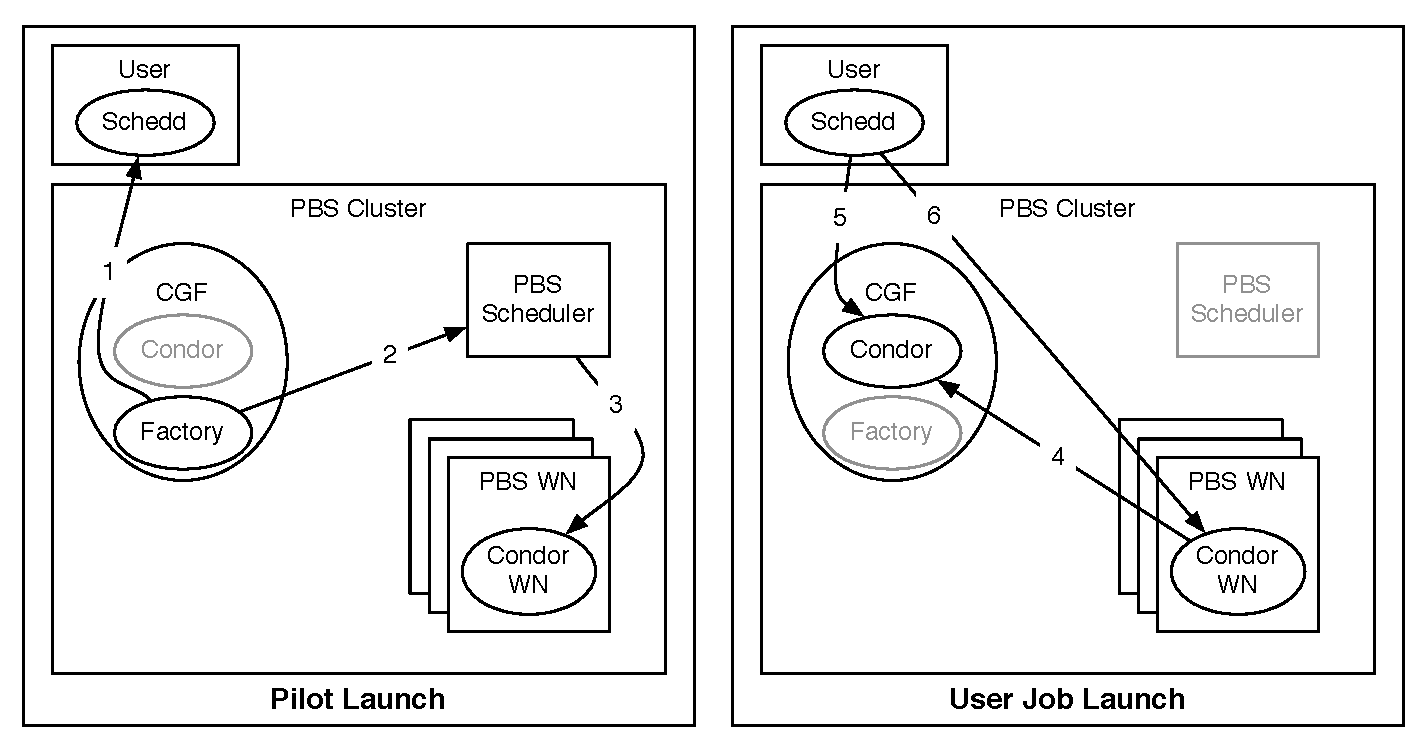
\includegraphics[scale=0.67]{images/CHEP-CGF}
\caption{Overview of the Campus Grid Factory}
\label{fig:cgfoverview}
\end{center}
\end{figure}

The Campus Grid Factory overview is shown in Figure \ref{fig:cgfoverview}.  The factory software starts by querying all 
the Condor schedd's on the campus to determine if they have jobs to run (1).  If idle jobs are found, the factory will 
submit (2) a pilot job for execution to the PBS scheduler.  When PBS resources are available, PBS will start the pilot 
job (3) on an execute host, which is a Condor worker node.  After starting, the Condor worker node will contact (4) the 
Condor installation at the CGF and list itself as a node available to run jobs.  This is the ``pilot launch" sequence.

To launch user jobs, the user schedd will first advertise (5) it is has idle jobs to run on the CGF's Condor collector.  
The CGF Condor negotiator matches the resources and orchestrates a direct connection (6) between the execute and 
submit hosts, running the user job.

Note the CGF and the overlay worker nodes create a Condor pool from the PBS cluster.  The factory collector will route 
jobs from other clusters to these available glideins just as it would for an all-condor cluster.

There are many architectural similarities between the CGF and GlideinWMS teams.  However, GlideinWMS was not chosen to 
run the CGF as the GlideinWMS is designed to have one central factory and a frontend on each submit host.  Therefore, 
if a non-Condor cluster becomes disconnected from the factory, even jobs that are submitted on the local cluster will 
be unable to run on the cluster since the factory cannot reach it, violating the decentralization goal.  The current 
CGF merges the roles of the frontend and factory in the GlideinWMS architecture, removing some complexity from the 
submit host.  At the core of GlideinWMS is the use of GSI for security; while HCC uses GSI security for its OSG work, 
we want to avoid making it a requirement for the campus.

The GlideinWMS system does a superior job of preparing and validating runtime environments compared to the CGF, an 
essential element for removing a common source of grid frustration.  However, we believe the runtime environment 
problem is mitigated on campuses because of the smaller number of resources and the closer working relationships 
between system administrators.
 
% \begin{figure}[htbp]
%\begin{center}
%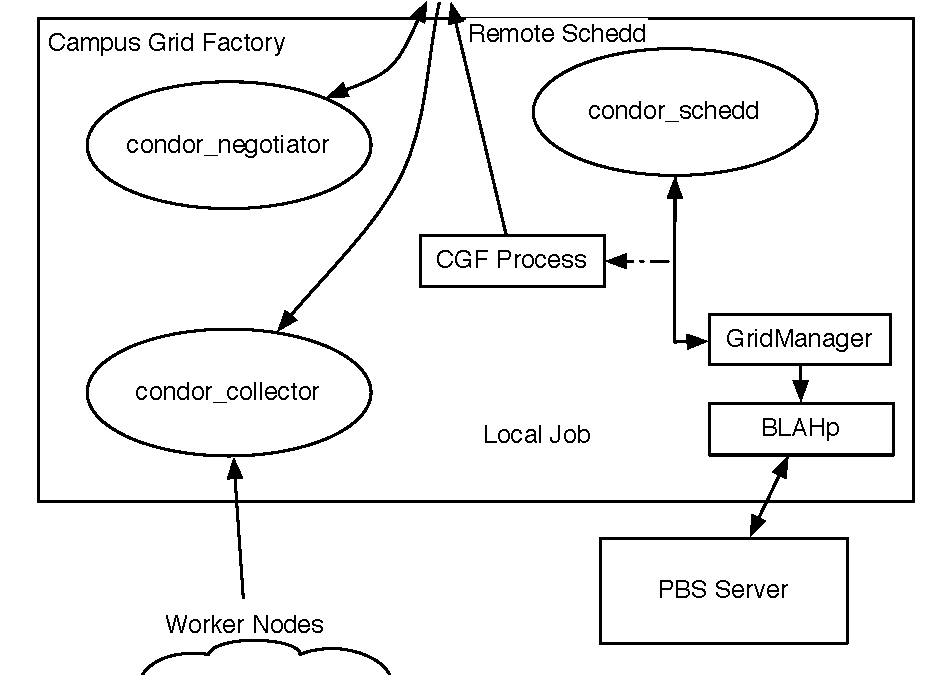
\includegraphics[scale=0.7]{images/CGF-Close}
%\caption{The Campus Grid Factory components.}
%\label{fig:cgfcomponents}
%\end{center}
%\end{figure}


\section{Bridging outside the campus \label{sec:bridging}}
There are two methods for expanding the campus grid described in Section \ref{sec:hcc}: through GlideinWMS to the OSG, 
or by linking campus grids through flocking.  The benefits of bridging externally are obvious - increased throughput 
for the local user's jobs.  HCC has been able to utilize over 7,000 remote job slots at a time, and has been able to 
bridge to all the campus grids discussed in Section \ref{sec:others}.  We connect to FermiGrid and GLOW through the OSG and 
to Purdue via Condor flocking.

Unlike the OSG, where the trust relationship is well-defined and common between sites, trust is established between 
campuses with flocking on a case-by-case basis.
The current model for trust is based on limited trusted hosts.  Each site publishes a list of submit and negotiator 
hosts that are trusted to submit and accept jobs, respectively.  This implicitly trusts an entire campus, while the OSG 
trust model is based on virtual organizations that may have no relationship to a physical campus or submit host.

The full campus grid architecture, with bridging, is shown in Figure \ref{fig:campusgrid}.  In this campus grid, the 
user first submits jobs to the local condor cluster (1).  If the local cluster can fulfill the user's needs, then the 
jobs will remain there.  If the local cluster is full or cannot meet the user's demand, Condor flocking will start 
submitting jobs to other campus clusters (2), either Condor or CGF-based.  If the on-campus 
resources are unable to meet the user's request, the local Condor schedd will expand its reach again (3) by looking 
outside the campus.  The jobs can also be sent to the OSG via flocking to a GlideinWMS 
frontend, which creates an overlay pool of grid resources.  In this architecture, every effort is given to find 
resources for the user (local, across campus, or externally), while maintaining the same vanilla Condor interface.

It is important to note the ever-widening circle of resources expands from the locality of the user.  It goes from the resource 
the user knows best (and has the best support for) to the most foreign one.  This is a very natural progression, and 
each step described comes with more complexity, and new failure modes.  If the user is ever frustrated at one 
transition, he can just remain contented with the resources he has, as opposed to having to switch between ``local 
mode" and ``grid mode".  Another usability boost is that all end-user interfaces are Condor vanilla universe.  The user 
never encounters errors translated between systems (a common user frustration) and the user needs to develop expertise 
in Condor alone.

\begin{figure}[htbp]
\begin{center}
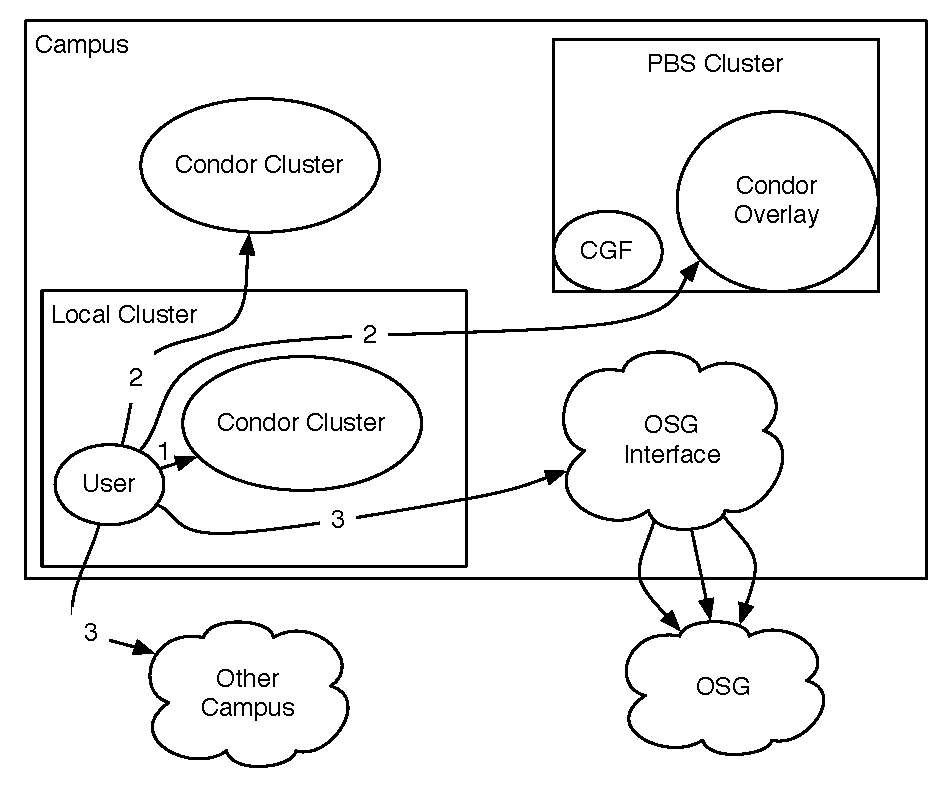
\includegraphics[scale=0.7]{images/CHEP-Campus}
\caption{The HCC Campus Grid architecture, complete with connections to other campuses and the OSG.  As each resource 
becomes fully utilized, the user's jobs will extend out to increasingly remote clusters.}
\label{fig:campusgrid}
\end{center}
\end{figure}


\section{Conclusions \label{sec:conclusions}}
The HTC philosophy can be a significant asset for campuses.  It improves utilization and gives user jobs better 
mobility.  The Open Science Grid has validated at a nationwide level and campuses including FermiGrid, GLOW, and Purdue 
have shown different methodologies for scaling grid-based HTC to the campus level.  These campus grid solutions can be 
categorized by how they implement the characteristics discussed in Section \ref{sec:requirements}.  HCC has been able 
to build on these previous ideas for a campus grid and improve on them using the Campus Grid Factory for non-Condor 
clusters.  We have shown these approaches can successfully bridge out to external grids.

HCC and OSG plans to continue to build on the CGF as a platform for integrating non-Condor clusters.  Over the next 
year, we plan on deploying it on other sites to establish new grids.  As noted, we hope to deploy improved data 
management strategies.  We also hope to more efficiently launch pilot jobs; in Figure \ref{fig:cgfoverview}, the 
factory currently queries the user schedd to determine if there are waiting jobs, and launching pilots if jobs are 
waiting.  We believe this model will lead to unused pilots in some cases, and can be improved.

\section{Acknowledgments}
This research was done using resources provided by the Open Science Grid,
which is supported by the National Science Foundation and the U.S.
Department of Energy's Office of Science.

%\bibliographystyle{amsplain}
\section*{References}
\bibliographystyle{iopart-num}
\bibliography{CampusGridCHEP}


\end{document}
